% Options for packages loaded elsewhere
\PassOptionsToPackage{unicode}{hyperref}
\PassOptionsToPackage{hyphens}{url}
%
\documentclass[
]{article}
\usepackage{amsmath,amssymb}
\usepackage{lmodern}
\usepackage{iftex}
\ifPDFTeX
  \usepackage[T1]{fontenc}
  \usepackage[utf8]{inputenc}
  \usepackage{textcomp} % provide euro and other symbols
\else % if luatex or xetex
  \usepackage{unicode-math}
  \defaultfontfeatures{Scale=MatchLowercase}
  \defaultfontfeatures[\rmfamily]{Ligatures=TeX,Scale=1}
\fi
% Use upquote if available, for straight quotes in verbatim environments
\IfFileExists{upquote.sty}{\usepackage{upquote}}{}
\IfFileExists{microtype.sty}{% use microtype if available
  \usepackage[]{microtype}
  \UseMicrotypeSet[protrusion]{basicmath} % disable protrusion for tt fonts
}{}
\makeatletter
\@ifundefined{KOMAClassName}{% if non-KOMA class
  \IfFileExists{parskip.sty}{%
    \usepackage{parskip}
  }{% else
    \setlength{\parindent}{0pt}
    \setlength{\parskip}{6pt plus 2pt minus 1pt}}
}{% if KOMA class
  \KOMAoptions{parskip=half}}
\makeatother
\usepackage{xcolor}
\usepackage[margin=1in]{geometry}
\usepackage{graphicx}
\makeatletter
\def\maxwidth{\ifdim\Gin@nat@width>\linewidth\linewidth\else\Gin@nat@width\fi}
\def\maxheight{\ifdim\Gin@nat@height>\textheight\textheight\else\Gin@nat@height\fi}
\makeatother
% Scale images if necessary, so that they will not overflow the page
% margins by default, and it is still possible to overwrite the defaults
% using explicit options in \includegraphics[width, height, ...]{}
\setkeys{Gin}{width=\maxwidth,height=\maxheight,keepaspectratio}
% Set default figure placement to htbp
\makeatletter
\def\fps@figure{htbp}
\makeatother
\setlength{\emergencystretch}{3em} % prevent overfull lines
\providecommand{\tightlist}{%
  \setlength{\itemsep}{0pt}\setlength{\parskip}{0pt}}
\setcounter{secnumdepth}{-\maxdimen} % remove section numbering
\newlength{\cslhangindent}
\setlength{\cslhangindent}{1.5em}
\newlength{\csllabelwidth}
\setlength{\csllabelwidth}{3em}
\newlength{\cslentryspacingunit} % times entry-spacing
\setlength{\cslentryspacingunit}{\parskip}
\newenvironment{CSLReferences}[2] % #1 hanging-ident, #2 entry spacing
 {% don't indent paragraphs
  \setlength{\parindent}{0pt}
  % turn on hanging indent if param 1 is 1
  \ifodd #1
  \let\oldpar\par
  \def\par{\hangindent=\cslhangindent\oldpar}
  \fi
  % set entry spacing
  \setlength{\parskip}{#2\cslentryspacingunit}
 }%
 {}
\usepackage{calc}
\newcommand{\CSLBlock}[1]{#1\hfill\break}
\newcommand{\CSLLeftMargin}[1]{\parbox[t]{\csllabelwidth}{#1}}
\newcommand{\CSLRightInline}[1]{\parbox[t]{\linewidth - \csllabelwidth}{#1}\break}
\newcommand{\CSLIndent}[1]{\hspace{\cslhangindent}#1}
\usepackage{setspace}\doublespacing
\usepackage{lineno}\linenumbers
\usepackage{booktabs}
\usepackage{longtable}
\usepackage{array}
\usepackage{multirow}
\usepackage{wrapfig}
\usepackage{float}
\usepackage{colortbl}
\usepackage{pdflscape}
\usepackage{tabu}
\usepackage{threeparttable}
\usepackage{threeparttablex}
\usepackage[normalem]{ulem}
\usepackage{makecell}
\usepackage{xcolor}
\ifLuaTeX
  \usepackage{selnolig}  % disable illegal ligatures
\fi
\IfFileExists{bookmark.sty}{\usepackage{bookmark}}{\usepackage{hyperref}}
\IfFileExists{xurl.sty}{\usepackage{xurl}}{} % add URL line breaks if available
\urlstyle{same} % disable monospaced font for URLs
\hypersetup{
  pdftitle={XXX},
  hidelinks,
  pdfcreator={LaTeX via pandoc}}

\title{XXX}
\author{}
\date{\vspace{-2.5em}}

\begin{document}
\maketitle

\begin{center}
\textbf{ORDER TBD:  H{\'{e}}ctor Tejero-Cicu{\'{e}}ndez$^{1,*}$,  Iris Men{\'{e}}ndez$^{2,3}$, Salvador Carranza$^{1}$, and Dean C. Adams$^{4}$} 
\end{center}

\begin{center}21 September, 2022\end{center}

\(^{1}\)Institute of Evolutionary Biology (CSIC-Universitat Pompeu
Fabra), Passeig Marítim de la Barceloneta 37-49, Barcelona 08002, Spain

\(^{2}\)Departamento de Geodinámica, Estratigrafía y Paleontología,
Facultad de Ciencias Geológicas, Universidad Complutense de Madrid,
C/José Antonio Novais 12, Madrid 28040, Spain

\(^{3}\)Departamento de Cambio Medioambiental, Instituto de Geociencias
(UCM, CSIC), C/Severo Ochoa 7, Madrid 28040, Spain

\(^{4}\)Department of Ecology, Evolution, and Organismal Biology, Iowa
State University, Ames, Iowa, 50010 USA

\(^{*}\)Correspondence: Héctor Tejero-Cicuéndez
\href{mailto:cicuendez93@gmail.com}{\nolinkurl{cicuendez93@gmail.com}}

\hfill\break

\textbf{Keywords}: Phenotypic Evolution, Morphospace, Allometry,
\emph{Pristurus} geckos \hfill\break

\textbf{Short Title}: XXX \hfill\break

\textbf{Author Contributions}: All authors collaboratively developed the
concept and contributed to all portions of this manuscript. HT-C, IM,
and DCA performed the analyses. All authors approve of the final product
and are willingly accountable for any portion of the
content.\hfill\break

\textbf{Conflicts of Interests}: The authors declare no conflicts of
interest.\hfill\break

\textbf{Data Archiving}: Data are available on DRYAD
(\url{doi:10.5061/dryad.xwdbrv1f6} (Tejero-Cicuéndez et al. 2021b)).
R-scripts are found in the Supplemental Information. \hfill\break

\textbf{Acknowledgments}: We thank XYZPDQ\ldots{} This work was
sponsored in part by XXX (to SC) DCA was funded in part by National
Science Foundation Grant DEB-2140720, and a Fulbright Senior Scholar
Grant.

\newpage

\hypertarget{abstract}{%
\section{Abstract}\label{abstract}}

asdf

\newpage

\hypertarget{introduction}{%
\section{Introduction}\label{introduction}}

some general paragraph on the evolution of phenotypic diversity
\hfill\break

when organisms colonize new and unique habitats, they are subjected to
novel ecological selection pressures in those habitats. Often these
selective pressures elicit changes in body form, as organisms adapt to
their new habitats (examples: some comment on ecomorphs, etc.). \ldots.
leads to so-called ecomorphs, with such well known examples in Anolis
lizards, cichlid fishes, etc. It follows that \ldots{} Some comment on
the fact that clades living in diverse ecological conditions often
display greater diversity in form and function (REFS).

However, while the above patterns have been well documented in a variety
of vertebrate taxa, what remains less known is how allometry plays a
role in this phenotypic diversification. We know that XYZPDQ (about
allometry). Then links to diversity..

The Afro-Arabian geckos in the genus \emph{Pristurus} afford the
opportunity to elucidate the interdigitating effects of allometry and
habitat specialization on clade-level patterns of phenotypic diversity.
Prior work on this system (Tejero-Cicuéndez et al. 2021a) has revealed
that \ldots{} (sentence or 2 about your prior study, getting to
diversity and \ldots{} Importantly, \ldots{} something about habitat.
\ldots. What remains unexamined however, is XYZPDQ\ldots{}

In this study, we \ldots{}

\hypertarget{materials-and-methods}{%
\section{Materials and Methods}\label{materials-and-methods}}

\hypertarget{data}{%
\subsection{Data}\label{data}}

For this study, we combined phenotypic, phylogenetic, and ecological
data to evaluate macroevolutionary trends in allometry, and to discern
the extent to which those patterns differed across species occupying
distinct ecological habitats. The data were obtained from our prior work
on this system (Tejero-Cicuéndez et al. 2021a, 2022), and are briefly
described here. First we used a time-dated, molecular phylogeny that
included all members of the genus \emph{Pristurus}, including several
currently undescribed taxa. The tree was estimated in a Bayesian
framework, using five mitochondrial markers, six nuclear markers, and 21
calibration points (for details see Tejero-Cicuéndez et al. 2022). Next
we categorized each species as belonging to one of three ecological
groups (ground, rock, or tree), based on descriptions in the literature
(see Tejero-Cicuéndez et al. 2021a). Finally, we obtained a phenotypic
data set containing body size (snout-vent length: SVL) and eight linear
measurements (\textbf{Figure 1}) that described overall body form: trunk
length (TrL), head length (HL), head width (HW), head height (HH),
humerus length (Lhu), ulna length (Lun), femur length (Lfe), and tibia
length (Ltb) (Tejero-Cicuéndez et al. 2021a). We restricted our study to
those species represented by five or more individuals; resulting in a
dataset of 687 individuals from 25 species (invidivuals per species:
\(\mu=27\); min = 9, max = 56). Species in the phenotypic dataset were
then matched to the phylogeny, which was subsequently pruned to arrive
at the final topology. All measurements were log-transformed prior to
statistical analyses. Additional details regarding data collection and
formal descriptions of each linear measurement may be found in the
original sources (see Tejero-Cicuéndez et al. 2021a, 2022). The data are
found on DRYAD: \url{https://doi.org/10.5061/dryad.xwdbrv1f6}
(Tejero-Cicuéndez et al. 2021b).

\hypertarget{statistical-analyses}{%
\subsection{Statistical Analyses}\label{statistical-analyses}}

We conducted a series of statistical analyses to interrogate allometric
trends, and macroevolutionary changes in allometry related to
diversification in body form. First, to determine whether allometric
trends in body form differed across habitat groups, we performed a
multivariate analysis of covariance, with body size (SVL), habitat, and
SVL*habitat as model effects. Significance was evaluated using 999
iterations of a permutation procedure, where residuals from a reduced
model were randomly permuted in each permutation (RRPP), model
statistics were recalculated, and used to generate empirical null
sampling distributions to evaluate the observed test statistics
(following Freedman and Lane 1983; Collyer and Adams 2007; Collyer et
al. 2015). Next we compared the multivariate allometric vectors for each
habitat group by calculating pairwise differences in their angular
direction in morphospace, and evaluating these relative to empirical
sampling distributions obtained through RRPP (Collyer and Adams 2007;
Adams and Collyer 2009; Collyer and Adams 2013). We then visualized
patterns of multivariate allometry relative to body size via regression
scores (Drake and Klingenberg 2008) and predicted lines (Adams and
Nistri 2010) based on fitted values from the linear model described
above. \hfill\break

Second, we examined changes in allometric trends across the phylogeny,
treating the head dimensions and limb dimensions separately. Because
both the head and limb data were multivariate, we accomplished this by
first performing a partial least squares analysis (Rohlf and Corti 2000)
of the head traits versus SVL, and the limb traits versus SVL, retaining
the PLS scores for each individual from the first dimension of this
analysis. Analysis of covariance was then used to obtain
species-specific slopes for \(PLS1_{head}\) vs.~SVL and \(PLS1_{limb}\)
vs.~SVL respectively, which represented the extent of head and limb
allometry within each species respectively. These were then mapped on
the phylogeny of \emph{Pristurus} using a Brownian motion model of
evolution, to qualitatively evaluate shifts in allometry across species
(for a similar approach see Adams and Nistri 2010). \hfill\break

Finally, to relate within-species allometric trends with patterns of
phenotypic diversification in the group we generated a phylomorphospace,
based on the size-standardized species means obtained from a
phylogenetic regression (see Tejero-Cicuéndez et al. 2021a). Here,
phenotypic similarities among species, relative to their phylognetic
relationships and habitat affiliations, were observed. All analyses were
conducted in R 4.2.1 (R Core Team 2022), using \texttt{RRPP} version
1.3.1 (Collyer and Adams 2018; Collyer and Adams 2022), and scripts
written by the authors (available at \textbf{XXX}).

\hypertarget{results}{%
\section{Results}\label{results}}

\hypertarget{discussion}{%
\section{Discussion}\label{discussion}}

\newpage

\hypertarget{references}{%
\section*{References}\label{references}}
\addcontentsline{toc}{section}{References}

\setlength{\parindent}{-0.25in} \setlength{\leftskip}{0.25in}
\setlength{\parskip}{8pt} \noindent

\hypertarget{refs}{}
\begin{CSLReferences}{1}{0}
\leavevmode\vadjust pre{\hypertarget{ref-AdamsCollyer2009}{}}%
Adams, D. C., and M. L. Collyer. 2009. A general framework for the
analysis of phenotypic trajectories in evolutionary studies. Evolution
63:1143--1154.

\leavevmode\vadjust pre{\hypertarget{ref-AdamsNistri2010}{}}%
Adams, D. C., and A. Nistri. 2010. Ontogenetic convergence and evolution
of foot morphology in european cave salamanders (family:
plethodontidae). BMC Evolutionary Biology 10:1--10. BioMed Central.

\leavevmode\vadjust pre{\hypertarget{ref-CollyerAdams2007}{}}%
Collyer, M. L., and D. C. Adams. 2007. Analysis of two-state
multivariate phenotypic change in ecological studies. Ecology
88:683--692.

\leavevmode\vadjust pre{\hypertarget{ref-CollyerAdams2013}{}}%
Collyer, M. L., and D. C. Adams. 2013. Phenotypic trajectory analysis:
Comparison of shape change patterns in evolution and ecology. Hystrix
24:75--83.

\leavevmode\vadjust pre{\hypertarget{ref-RRPP}{}}%
Collyer, M. L., and D. C. Adams. 2022.
\href{https://CRAN.R-project.org/package=RRPP}{R: RRPP: Linear model
evaluation with randomized residuals in a permutation procedure. Vsn.
1.3.1}. R Foundation for Statistical Computing, Vienna, Austria.

\leavevmode\vadjust pre{\hypertarget{ref-CollyerAdams2018}{}}%
Collyer, M. L., and D. C. Adams. 2018. RRPP: An r package for fitting
linear models to high-dimensional data using residual randomization.
Methods in Ecology and Evolution 9:1772--1779.

\leavevmode\vadjust pre{\hypertarget{ref-Collyer_et_al2015}{}}%
Collyer, M. L., D. J. Sekora, and D. C. Adams. 2015. A method for
analysis of phenotypic change for phenotypes described by
high-dimensional data. Heredity 115:357--365.

\leavevmode\vadjust pre{\hypertarget{ref-DrakeKlingenberg2008}{}}%
Drake, A. G., and C. P. Klingenberg. 2008.
\href{https://doi.org/10.1098/rspb.2007.1169}{The pace of morphological
change: Historical transformation of skull shape in st bernard dogs}.
Proceedings of the Royal Society B: Biological Sciences 275:71--76.

\leavevmode\vadjust pre{\hypertarget{ref-Freedman1983}{}}%
Freedman, D., and D. Lane. 1983. A nonstochastic interpretation of
reported significance levels. Journal of Business {\&} Economic
Statistics 1:292--298.

\leavevmode\vadjust pre{\hypertarget{ref-RCT}{}}%
R Core Team. 2022. \href{https://www.R-project.org/}{R: A language and
environment for statistical computing. Version 4.2.1}. R Foundation for
Statistical Computing, Vienna, Austria.

\leavevmode\vadjust pre{\hypertarget{ref-Rohlf2000}{}}%
Rohlf, F. J., and M. Corti. 2000. Use of two-block partial least-squares
to study covariation in shape. Systematic Biology 49:740--753.

\leavevmode\vadjust pre{\hypertarget{ref-Tejero-Cicuendez2022}{}}%
Tejero-Cicuéndez, H., A. H. Patton, D. S. Caetano, J. Šmíd, L. J.
Harmon, and S. Carranza. 2022. Reconstructing squamate biogeography in
afro-arabia reveals the influence of a complex and dynamic geologic
past. Systematic Biology 71:261--272.

\leavevmode\vadjust pre{\hypertarget{ref-Tejero-Cicuendez2021}{}}%
Tejero-Cicuéndez, H., M. Simó-Riudalbas, I. Menéndez, and S. Carranza.
2021a. \href{https://doi.org/10.1098/rspb.2021.1821}{Ecological
specialization, rather than the island effect, explains morphological
diversification in an ancient radiation of geckos}. Proceedings of the
Royal Society B: Biological Sciences 288:20211821.

\leavevmode\vadjust pre{\hypertarget{ref-PristurusData}{}}%
Tejero-Cicuéndez, H., M. Simó-Riudalbas, I. Menéndez, and S. Carranza.
2021b. Ecological specialization, rather than the island effect,
explains morphological diversification in an ancient radiation of
geckos. Dryad digital repository. (Doi:10.5061/dryad.xwdbrv1f6).

\end{CSLReferences}

\newpage

\hypertarget{figures}{%
\section{Figures}\label{figures}}

Figure 1. Linear Measurements used in this study. SVL = snout-vent
length, TL = trunk length, HL = head length, HW = head width, HH = head
height, Lhu = humerus length, Lun = ulna length, Lfe = femur length, Ltb
= tibia length (for details see Tejero-Cicuéndez et al. 2021a).
\hfill\break

Figure 2. Plot of regression scores and predicted lines representing the
relationship between linear body measurements and size (SVL).
Individuals re colored by habitat use: rock (beige), ground (dark
purple), and tree (magenta). \hfill\break

Figure 3. Traitgrams showing the evolution of body size (SVL) through
time based on the phylogenetic tree of \emph{Pristurus}. Colors
represent an evolutionary mapping of regression slopes describing the
relationship of (A) head morphology versus body size, and (B) limb
proportions versus body size (see text for descriptions). Species names
are colored by habitat use: rock (beige), ground (dark purple), and tree
(magenta). \hfill\break

Figure 4. Phylomorphospace of \emph{Pristurus}, based on residuals from
a phylogenetic regression of body measurements on size (SVL). Species
means are colored by habitat use: rock (beige), ground (dark purple),
and tree (magenta). Large and small rock-dwelling and ground-dwelling
are highlighted with darker colors to highlight their differentiation
and relative positions in morphospace.

\newpage

\begin{figure}

{\centering 
\includegraphics[width=1\linewidth]{Figs/Fig1} 

}

\caption{Linear Measurements used in this study. SVL = snout-vent length, TL = trunk length, HL = head length, HW = head width, HH = head height, Lhu = humerus length, Lun = ulna length, Lfe = femur length, Ltb = tibia length (for details see Tejero-Cicu{'{e}}ndez et al. 2021a).}\label{fig:unnamed-chunk-1}
\end{figure}

\newpage

\begin{figure}
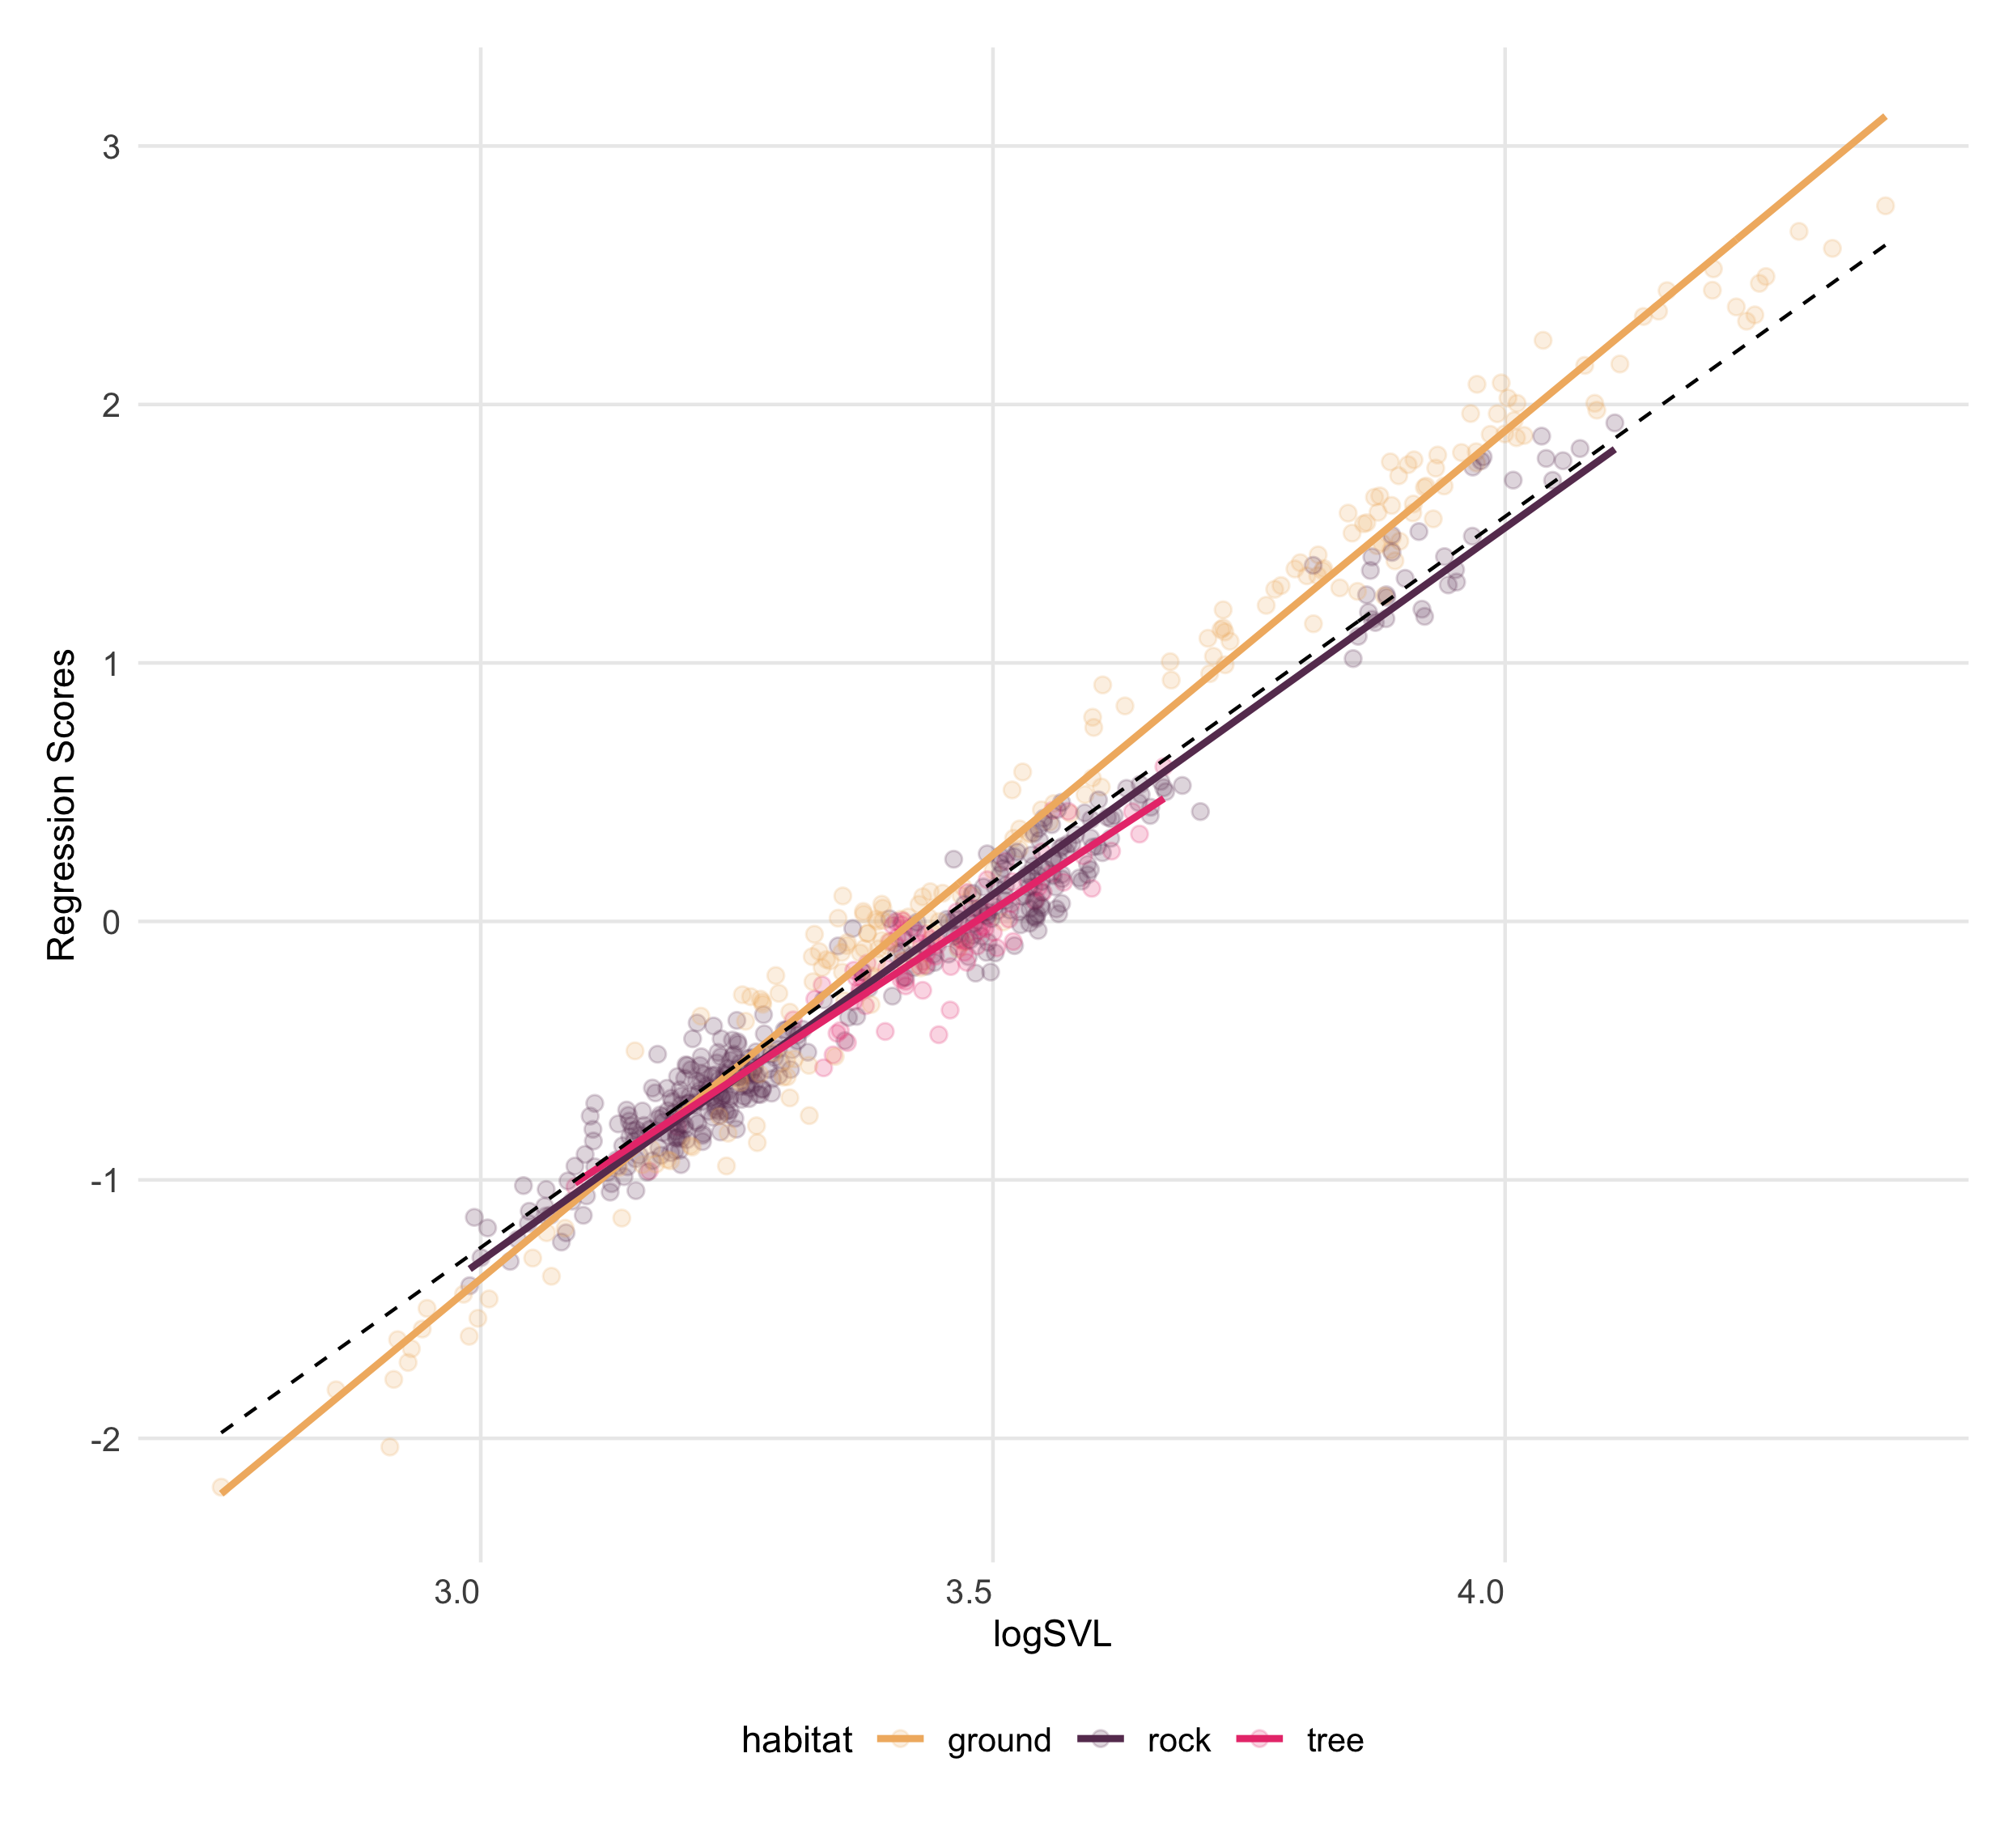
\includegraphics[width=1\linewidth]{Figs/figure_2_ggplot} \caption{Plot of regression scores and predicted lines representing the relationship between linear body measurements and size (SVL). Individuals re colored by habitat use: rock (beige), ground (dark purple), and tree (magenta).}\label{fig:unnamed-chunk-2}
\end{figure}

\newpage

\begin{figure}
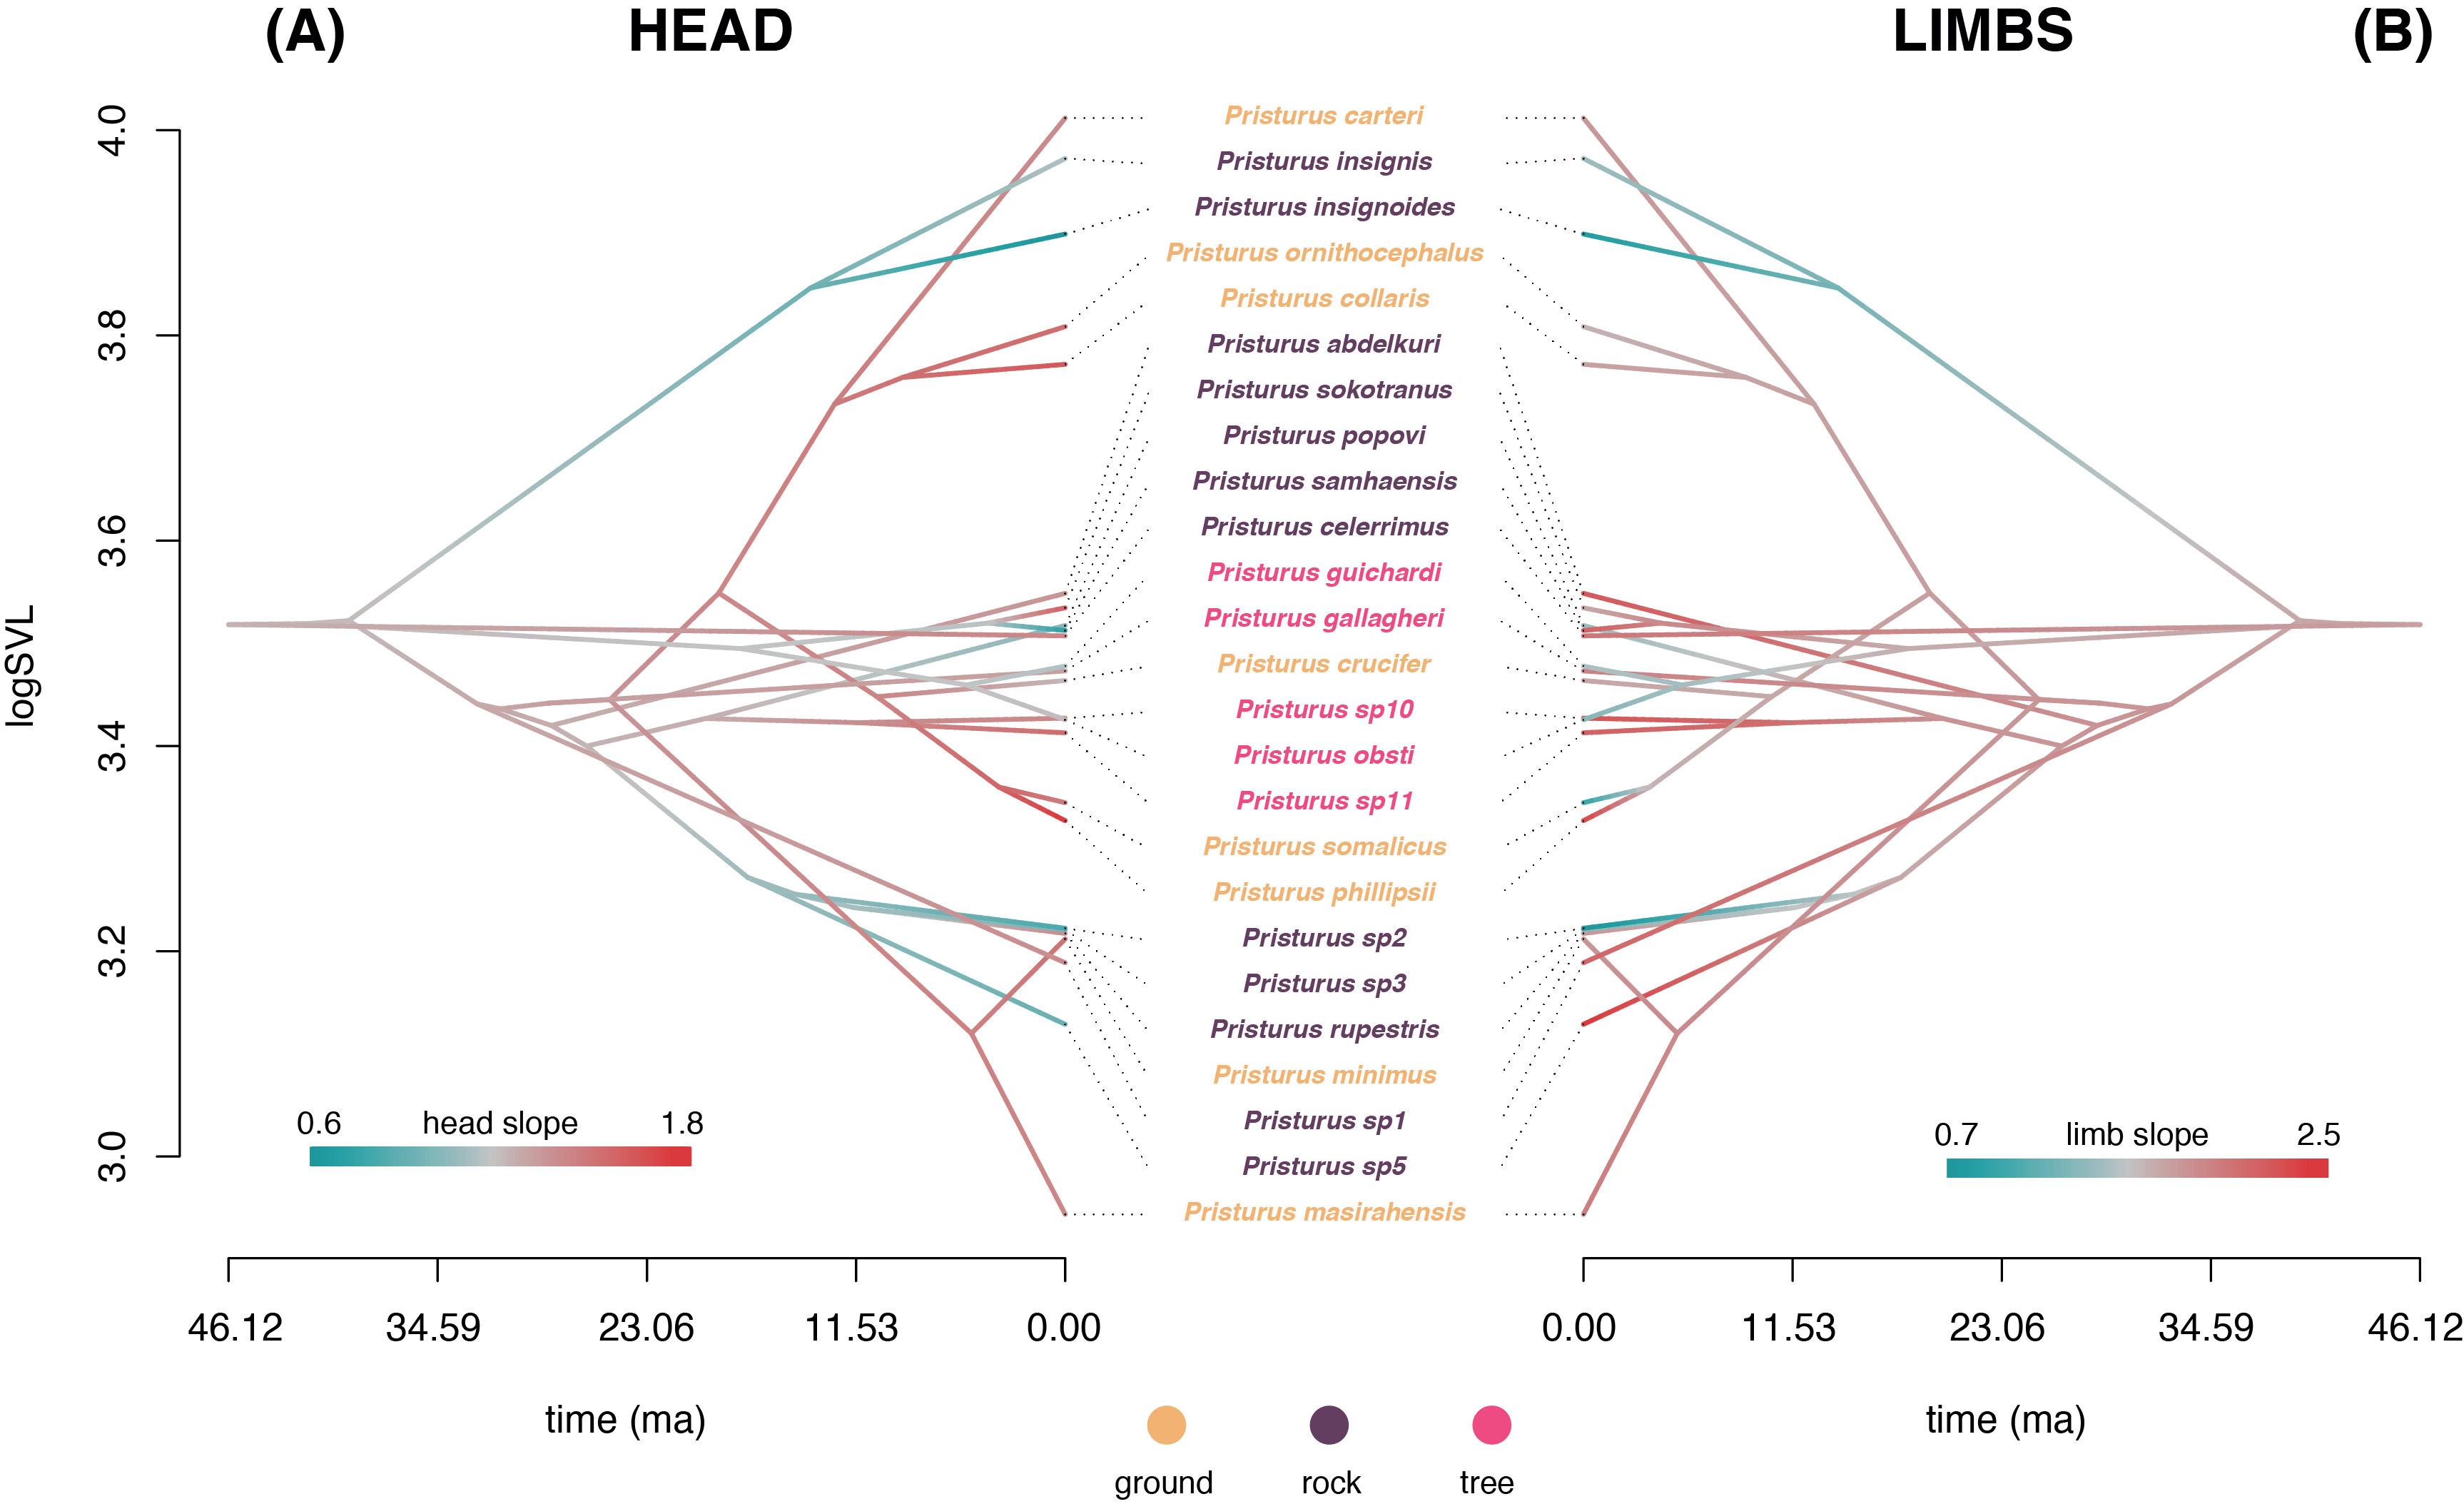
\includegraphics[width=1\linewidth]{Figs/figure_phenograms} \caption{Traitgrams showing the evolution of body size (SVL) through time based on the phylogenetic tree of \textit{Pristurus}. Colors represent an evolutionary mapping of regression slopes describing the relationship of (A) head morphology versus body size, and (B) limb proportions versus body size (see text for descriptions). Species names are colored by habitat use: rock (beige), ground (dark purple), and tree (magenta).}\label{fig:unnamed-chunk-3}
\end{figure}

\newpage

\begin{figure}
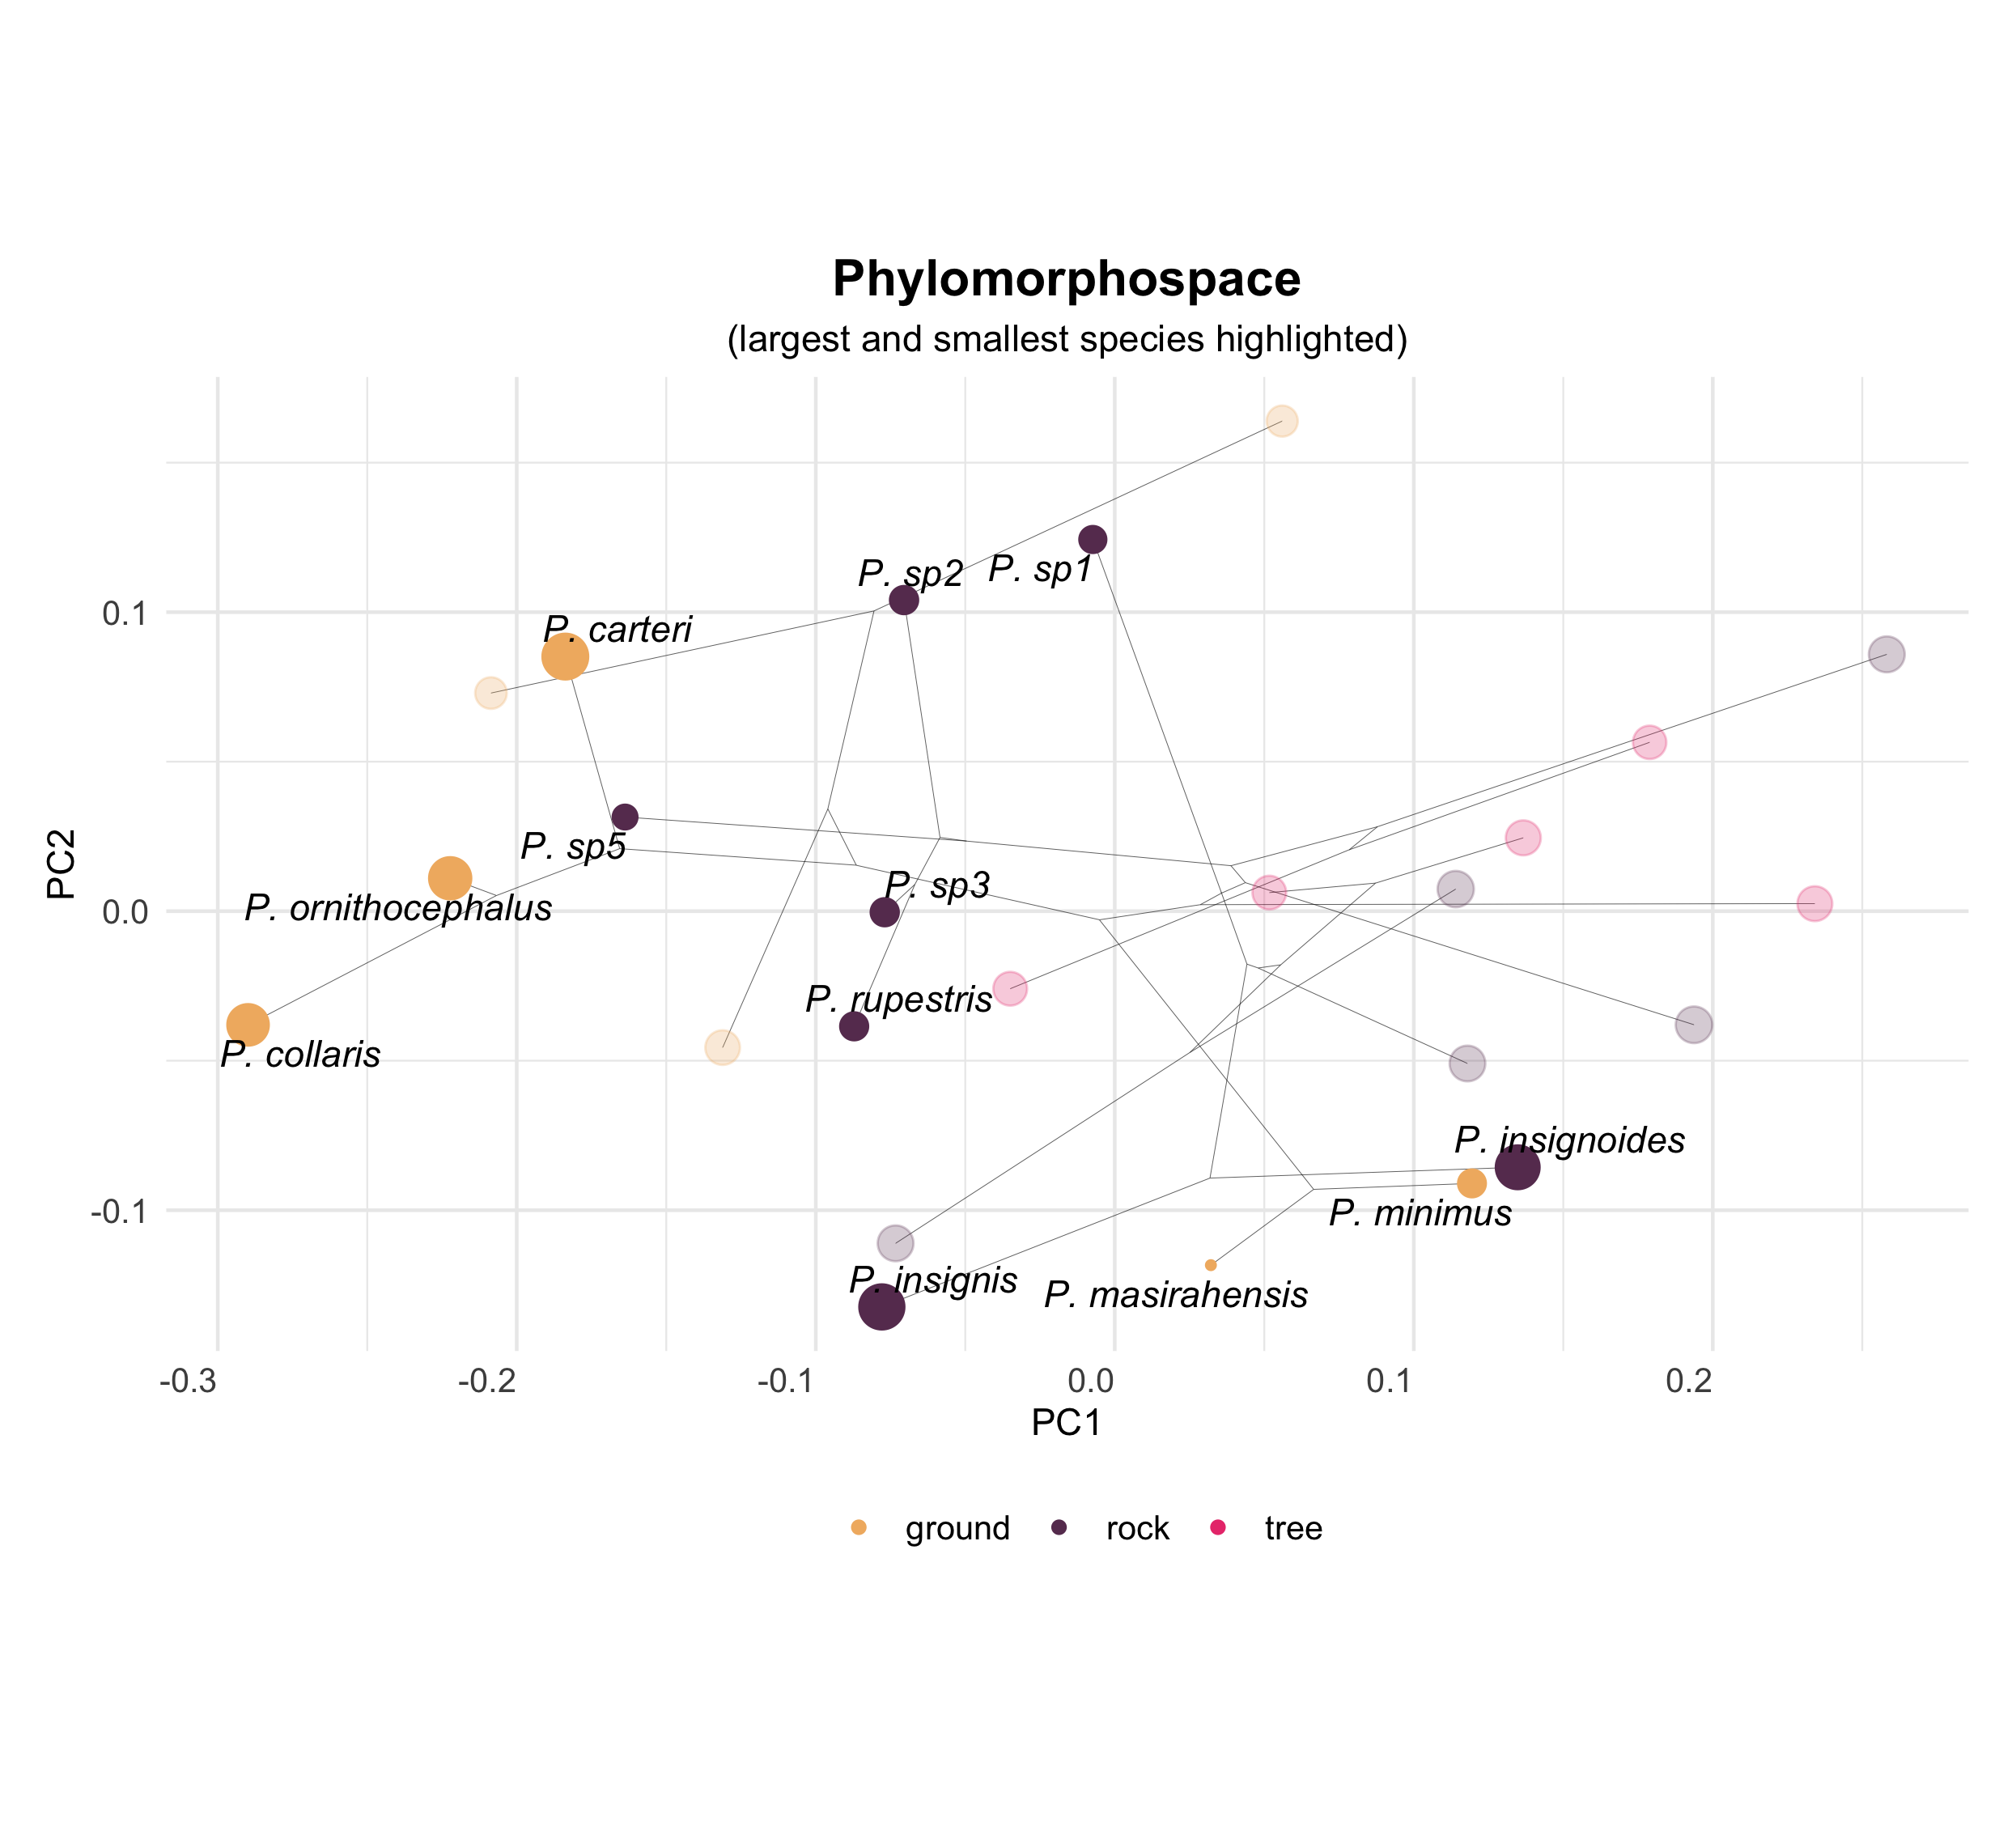
\includegraphics[width=1\linewidth]{Figs/phylomorphospace_large_small} \caption{Phylomorphospace of \textit{Pristurus}, based on residuals from a phylogenetic regression of body measurements on size (SVL). Species means are colored by habitat use: rock (beige), ground (dark purple), and tree (magenta). Large and small rock-dwelling and ground-dwelling are highlighted with darker colors to highlight their differentiation and relative positions in morphospace.}\label{fig:unnamed-chunk-4}
\end{figure}

\end{document}
